\documentclass[10pt,a4paper]{article}

\usepackage[utf8]{inputenc}
\usepackage[T1]{fontenc}
\usepackage[a4paper,margin=0.6in,top=0.52in,bottom=0.52in]{geometry}
\usepackage{tikz}
\usetikzlibrary{shapes,arrows,positioning,calc,fit,backgrounds}
\usepackage{xcolor}
\usepackage{lmodern}
\usepackage{booktabs}
\usepackage{tabularx}
\usepackage{enumitem}
\usepackage{titlesec}
\usepackage{fancyhdr}
\usepackage{listings}
\usepackage{microtype}
\usepackage[colorlinks=true,linkcolor=primary,urlcolor=secondary]{hyperref}

% =========================================================
% Palette & Styling (Matching lab_2.tex)
% =========================================================
\definecolor{primary}{RGB}{24, 43, 73}        % Deep clean navy
\definecolor{secondary}{RGB}{14, 116, 144}   % Teal accent
\definecolor{darkslate}{RGB}{30, 41, 59}     % Normal text color
\definecolor{boxbg}{RGB}{248, 250, 252}      % Soft light box
\definecolor{bordergray}{RGB}{226, 232, 240} % Light border

% Terminal Color Scheme: Modern Light Grey Theme
\definecolor{termbg}{RGB}{246, 248, 250}     % Light grey terminal body
\definecolor{termbar}{RGB}{229, 231, 235}    % Medium light grey title bar
\definecolor{termborder}{RGB}{209, 213, 219} % Crisp border line
\definecolor{termtext}{RGB}{31, 41, 55}      % Dark charcoal text
\definecolor{termuser}{RGB}{22, 101, 52}     % Dark green for user
\definecolor{termhost}{RGB}{21, 128, 61}     % Green for host
\definecolor{termpath}{RGB}{29, 78, 216}     % Blue for directory path
\definecolor{termcmd}{RGB}{17, 24, 39}       % Bold black for commands
\definecolor{termout}{RGB}{55, 65, 81}       % Clear dark grey for outputs
\definecolor{termdir}{RGB}{37, 99, 235}      % Blue for directories
\definecolor{termfile}{RGB}{31, 41, 55}      % Dark for regular files
\definecolor{termhidden}{RGB}{107, 114, 128} % Muted grey
\definecolor{termsize}{RGB}{180, 83, 9}      % Amber for sizes
\definecolor{termperm}{RGB}{79, 70, 229}     % Indigo for permissions

% Code Listing Colors
\definecolor{codebg}{RGB}{248, 250, 252}
\definecolor{codeborder}{RGB}{218, 224, 233}
\definecolor{codekw}{RGB}{14, 116, 144}
\definecolor{codestr}{RGB}{22, 101, 52}
\definecolor{codecomment}{RGB}{100, 116, 139}
\definecolor{codenum}{RGB}{148, 163, 184}

% Table helpers
\newcolumntype{Y}{>{\centering\arraybackslash}X}

% =========================================================
% Section Headings
% =========================================================
\titleformat{\section}
  {\color{primary}\large\bfseries\sffamily\raggedright}
  {\thesection.}{0.5em}{}
\titlespacing*{\section}{0pt}{7pt}{2pt}

\titleformat{\subsection}
  {\color{secondary}\normalsize\bfseries\sffamily\raggedright}
  {\thesubsection}{0.5em}{}
\titlespacing*{\subsection}{0pt}{5pt}{2pt}

% =========================================================
% Headers and Footers
% =========================================================
\pagestyle{fancy}
\fancyhf{}
\renewcommand{\headrulewidth}{0.4pt}
\renewcommand{\footrulewidth}{0pt}
\fancyhead[L]{\small\sffamily\color{darkslate} Operating Systems Lab}
\fancyhead[R]{\small\sffamily\color{darkslate} Lab Report: SJF Scheduling Algorithm}
\fancyfoot{}

\fancypagestyle{firstpage}{%
  \fancyhf{}
  \renewcommand{\headrulewidth}{0pt}
  \renewcommand{\footrulewidth}{0pt}
}

% =========================================================
% Terminal Window Macro
% =========================================================
\newcommand{\termprompt}[1][\textasciitilde]{%
  \textbf{\textcolor{termuser}{ratul}}\textcolor{termtext}{@}\textbf{\textcolor{termhost}{firefly}}\textcolor{termtext}{:}\textbf{\textcolor{termpath}{#1}}\textcolor{termcmd}{\$}\ %
}

\newcommand{\terminalwindow}[3][\dimexpr\linewidth-0.6pt\relax]{%
\par\vspace{2pt}%
{\centering
\begin{tikzpicture}
  % 1. Terminal text on main layer
  \node[
      text=termtext,
      font=\ttfamily\fontsize{7.2}{9.2}\selectfont,
      align=left,
      text width=\dimexpr#1-1.02cm\relax,
      inner xsep=6pt,
      inner ysep=6pt,
      anchor=north west
  ] (body) at (0.32cm, -0.56cm) {#3};

  % Coordinates
  \coordinate (topleft) at (0, 0);
  \coordinate (bottomright) at ($(body.south -| #1, 0) + (0, -5pt)$);
  \coordinate (titlecenter) at ($0.5*(topleft) + 0.5*(#1, 0) + (0, -0.28cm)$);

  % 2. Background and Title bar on background layer
  \begin{scope}[on background layer]
    \fill[termbg, rounded corners=6pt] (topleft) rectangle (bottomright);

    \begin{scope}
      \clip[rounded corners=6pt] (topleft) rectangle (bottomright);
      \fill[termbar] (topleft) rectangle (#1, -0.56cm);
      \draw[termborder, line width=0.5pt] (0, -0.56cm) -- (#1, -0.56cm);
    \end{scope}

    \draw[termborder, line width=0.6pt, rounded corners=6pt] (topleft) rectangle (bottomright);
  \end{scope}

  % 3. Window control dots
  \fill[red!80!black] (0.36cm, -0.28cm) circle (0.07cm);
  \fill[yellow!80!black] (0.63cm, -0.28cm) circle (0.07cm);
  \fill[green!75!black] (0.90cm, -0.28cm) circle (0.07cm);

  % 4. Centered terminal title
  \node[
      text=gray!40!black,
      font=\sffamily\bfseries\fontsize{7.2}{8}\selectfont,
      anchor=center
  ] at (titlecenter) {#2};
\end{tikzpicture}\par}%
\vspace{2pt}%
}

\newcommand{\cmd}[1]{\texttt{\textbf{#1}}}

% =========================================================
% Code Listing Configuration
% =========================================================
\lstset{
  language=C,
  backgroundcolor=\color{codebg},
  basicstyle=\ttfamily\fontsize{7.2}{9.0}\selectfont\color{darkslate},
  keywordstyle=\bfseries\color{codekw},
  commentstyle=\itshape\color{codecomment},
  stringstyle=\color{codestr},
  numbers=left,
  numberstyle=\tiny\color{codenum},
  stepnumber=1,
  numbersep=8pt,
  showstringspaces=false,
  breaklines=true,
  frame=single,
  rulecolor=\color{codeborder},
  tabsize=4,
  xleftmargin=14pt,
  framexleftmargin=14pt
}

\begin{document}
\raggedbottom
\thispagestyle{firstpage}

% =========================================================
% Title Block
% =========================================================
\begin{center}
  {\Large\bfseries\sffamily\color{primary} Experiment Title: Implementation of Shortest Job First (SJF) Non-Preemptive CPU Scheduling Algorithm}\\[3pt]
  {\normalsize\sffamily\textbf{Topic:} Non-Preemptive CPU Scheduling with Arrival Time in C}
\end{center}
\vspace{-4pt}

% =========================================================
% 1. Problem
% =========================================================
\section{Problem}
In multi-programmed operating systems, CPU scheduling determines the order in which processes execute. The objective of this lab is to implement the \textbf{Shortest Job First (SJF) Non-Preemptive} CPU scheduling algorithm in C.

The program must:
\begin{itemize}[noitemsep,topsep=1pt,leftmargin=1.2em]
  \item Accept the total number of processes ($n$), arrival time ($AT$), and burst time ($BT$) for each process.
  \item Schedule processes based on the shortest burst time among available processes.
  \item Handle different arrival times and break burst-time ties using first-come, first-served (FCFS) order.
  \item Compute Completion Time ($CT$), Turnaround Time ($TAT$), and Waiting Time ($WT$) for every process.
  \item Display the tabular summary, Total Turnaround Time, Total Waiting Time, Average $TAT$, and Average $WT$.
\end{itemize}

\subsection{Environment \& Tools}
\vspace{-2pt}
\begin{table}[h!]
\centering\footnotesize
\renewcommand{\arraystretch}{1.06}
\begin{tabularx}{\linewidth}{lXlX}
\toprule
\textbf{Item} & \textbf{Details} & \textbf{Item} & \textbf{Details} \\
\midrule
\textbf{Operating System} & Linux (Ubuntu 24.04 LTS) & \textbf{Host Machine} & \texttt{firefly} \\
\textbf{User Account} & \texttt{ratul} & \textbf{Language \& Standard} & C (GNU C99) \\
\textbf{Compiler} & GCC (\cmd{gcc 13.x}) & \textbf{Execution Shell} & GNU Bash 5.2 \\
\bottomrule
\end{tabularx}
\end{table}
\vspace{-6pt}

% =========================================================
% 2. Theoretical Solution
% =========================================================
\section{Theoretical Solution}
Shortest Job First (SJF) non-preemptive scheduling selects the process with the smallest execution (burst) time from the ready queue once the CPU becomes free.

\subsection{Key Principles}
\begin{itemize}[noitemsep,topsep=1pt,leftmargin=1.2em]
  \item \textbf{Non-Preemptive Nature:} Once the CPU is allocated to a process, it cannot be interrupted until it finishes its entire burst time.
  \item \textbf{Ready Queue Eligibility:} A process $i$ can only be chosen at time $T$ if it has already arrived ($AT_i \le T$).
  \item \textbf{Tie Breaking:} If two ready processes have the same burst time, the one with earlier arrival time is executed first.
  \item \textbf{CPU Idle State:} If no process is ready at the current time, the system advances time until a process arrives.
\end{itemize}

\subsection{Formulas}
For each process $i$, performance metrics are calculated using standard formulas:
\begin{itemize}[noitemsep,topsep=1pt,leftmargin=1.2em]
  \item \textbf{Turnaround Time ($TAT$):} Total time taken from arrival to completion:
  \[ TAT_i = CT_i - AT_i \]
  \item \textbf{Waiting Time ($WT$):} Total time spent waiting in the ready queue:
  \[ WT_i = TAT_i - BT_i \]
  \item \textbf{Average Turnaround Time ($Avg\_TAT$):} $\frac{\sum_{i=1}^{n} TAT_i}{n}$
  \item \textbf{Average Waiting Time ($Avg\_WT$):} $\frac{\sum_{i=1}^{n} WT_i}{n}$
\end{itemize}

\subsection{Gantt Chart Representation}
Figure 1 illustrates the non-preemptive timeline for 4 processes ($P_1$: $AT=0, BT=7$; $P_2$: $AT=2, BT=4$; $P_3$: $AT=4, BT=1$; $P_4$: $AT=5, BT=4$):

\begin{center}
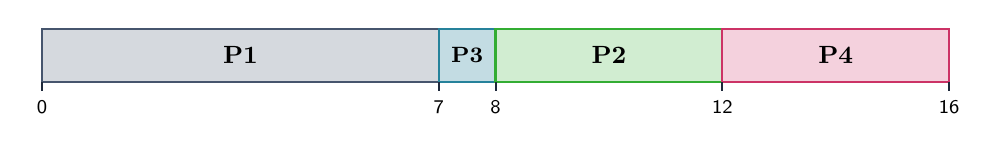
\begin{tikzpicture}[x=0.72cm, y=0.75cm]
  % P1
  \fill[primary!18] (0,0) rectangle (7,0.9);
  \draw[primary!80, line width=0.8pt] (0,0) rectangle (7,0.9);
  \node at (3.5, 0.45) {\bfseries\small P1};

  % P3
  \fill[secondary!25] (7,0) rectangle (8,0.9);
  \draw[secondary!90, line width=0.8pt] (7,0) rectangle (8,0.9);
  \node at (7.5, 0.45) {\bfseries\footnotesize P3};

  % P2
  \fill[green!60!black!18] (8,0) rectangle (12,0.9);
  \draw[green!60!black!80, line width=0.8pt] (8,0) rectangle (12,0.9);
  \node at (10, 0.45) {\bfseries\small P2};

  % P4
  \fill[purple!18] (12,0) rectangle (16,0.9);
  \draw[purple!80, line width=0.8pt] (12,0) rectangle (16,0.9);
  \node at (14, 0.45) {\bfseries\small P4};

  % Time markers
  \foreach \x in {0, 7, 8, 12, 16} {
    \draw[darkslate, line width=0.7pt] (\x, 0) -- (\x, -0.15);
    \node[below, font=\scriptsize\sffamily] at (\x, -0.15) {\x};
  }
\end{tikzpicture}
\vspace{-4pt}
\end{center}
\centerline{\footnotesize\textbf{Figure 1:} Gantt Chart of Non-Preemptive SJF Execution.}
\vspace{4pt}

\subsection{Algorithmic Approach}
\begin{enumerate}[noitemsep,topsep=1pt,leftmargin=1.4em]
  \item Read process count $n$, arrival times $arrival[i]$, and burst times $burst[i]$.
  \item Sort processes in ascending order of arrival time using selection sort.
  \item Initialize $current\_time = 0$ and $completed = 0$.
  \item Repeat while $completed < n$:
  \begin{itemize}[noitemsep,topsep=1pt,leftmargin=1.0em]
    \item Scan all uncompleted processes where $arrival[i] \le current\_time$.
    \item Select the one with the smallest $burst[i]$. If tied, select the smaller $arrival[i]$.
    \item If a process is found: $CT = current\_time + burst$, $TAT = CT - arrival$, $WT = TAT - burst$. Mark process complete, advance $current\_time = CT$, increment $completed$.
    \item If no process has arrived yet: advance $current\_time$ by 1 unit.
  \end{itemize}
  \item Compute average turnaround time and average waiting time.
\end{enumerate}

\newpage

% =========================================================
% 3. Expected Input/Output (I/O) Set
% =========================================================
\section{Expected Input/Output (I/O) Set}
The input consists of integer counts and positive values for arrival and burst times. The output provides the detailed schedule metrics and overall averages.

\subsection{Input Specification}
\begin{itemize}[noitemsep,topsep=1pt,leftmargin=1.2em]
  \item Total processes: $n = 4$
  \item Inputs per process: Process ID, Arrival Time ($AT$), Burst Time ($BT$).
\end{itemize}

\subsection{Tabular Input and Expected Output}
\vspace{-2pt}
\begin{table}[h!]
\centering\footnotesize
\renewcommand{\arraystretch}{1.08}
\begin{tabularx}{\linewidth}{YYYYYY}
\toprule
\textbf{Process} & \textbf{Arrival Time ($AT$)} & \textbf{Burst Time ($BT$)} & \textbf{Completion Time ($CT$)} & \textbf{Turnaround Time ($TAT$)} & \textbf{Waiting Time ($WT$)} \\
\midrule
\textbf{P1} & 0 & 7 & 7  & 7  & 0 \\
\textbf{P2} & 2 & 4 & 12 & 10 & 6 \\
\textbf{P3} & 4 & 1 & 8  & 4  & 3 \\
\textbf{P4} & 5 & 4 & 16 & 11 & 7 \\
\bottomrule
\end{tabularx}
\end{table}
\vspace{-6pt}

\subsection{Expected Summary Metrics}
\begin{itemize}[noitemsep,topsep=1pt,leftmargin=1.2em]
  \item \textbf{Total Turnaround Time:} $7 + 10 + 4 + 11 = 32$
  \item \textbf{Total Waiting Time:} $0 + 6 + 3 + 7 = 16$
  \item \textbf{Average Turnaround Time:} $32 / 4 = 8.00$
  \item \textbf{Average Waiting Time:} $16 / 4 = 4.00$
\end{itemize}

% =========================================================
% 4. Source Code
% =========================================================
\section{Source Code}
The complete C implementation of the Non-Preemptive SJF scheduling algorithm is given below:

\begin{lstlisting}
#include <stdio.h>

int main() {
    int n;

    printf("Enter the number of processes: ");
    scanf("%d", &n);

    int process[n], arrival[n], burst[n];
    int completion[n], turnaround[n], waiting[n];
    int is_completed[n];

    int i, j, temp, pos;
    int current_time = 0;
    int completed = 0;

    float totalTAT = 0;
    float totalWT = 0;
    float averageTAT, averageWT;

    // Input process details
    for (i = 0; i < n; i++) {
        process[i] = i + 1;

        printf("Enter arrival time of process %d: ", process[i]);
        scanf("%d", &arrival[i]);

        printf("Enter burst time of process %d: ", process[i]);
        scanf("%d", &burst[i]);

        completion[i] = -1;
        is_completed[i] = 0;
    }

    // Sorting processes based on arrival time
    for (i = 0; i < n; i++) {
        pos = i;

        for (j = i + 1; j < n; j++) {
            if (arrival[j] < arrival[pos]) {
                pos = j;
            }
        }

        // Swap arrival time
        temp = arrival[i];
        arrival[i] = arrival[pos];
        arrival[pos] = temp;

        // Swap burst time
        temp = burst[i];
        burst[i] = burst[pos];
        burst[pos] = temp;

        // Swap process ID
        temp = process[i];
        process[i] = process[pos];
        process[pos] = temp;
    }

    // Apply Shortest Job First (Non-Preemptive)
    while (completed != n) {

        int min_burst = 9999;
        int index = -1;

        // Find the shortest available process
        for (i = 0; i < n; i++) {

            if (arrival[i] <= current_time && is_completed[i] == 0) {

                if (burst[i] < min_burst) {
                    min_burst = burst[i];
                    index = i;
                }

                // If burst times are equal, select the one
                // that arrived first
                else if (burst[i] == min_burst &&
                         arrival[i] < arrival[index]) {
                    index = i;
                }
            }
        }

        // If a process is available
        if (index != -1) {

            completion[index] = current_time + burst[index];
            turnaround[index] = completion[index] - arrival[index];
            waiting[index] = turnaround[index] - burst[index];

            // Add to totals
            totalTAT = totalTAT + turnaround[index];
            totalWT = totalWT + waiting[index];

            // Update current time
            current_time = completion[index];

            is_completed[index] = 1;
            completed++;
        }

        // If no process has arrived yet
        else {
            current_time++;
        }
    }

    // Calculate averages
    averageTAT = totalTAT / n;
    averageWT = totalWT / n;

    // Printing the final process table
    printf("\nProcess\tArrival Time\tBurst Time\tCompletion Time\tTurnaround Time\tWaiting Time\n");

    for (i = 0; i < n; i++) {
        printf("P%d\t%d\t\t%d\t\t%d\t\t%d\t\t%d\n",
               process[i],
               arrival[i],
               burst[i],
               completion[i],
               turnaround[i],
               waiting[i]);
    }

    // Print total and average values
    printf("\nTotal Turnaround Time = %.0f", totalTAT);
    printf("\nTotal Waiting Time    = %.0f", totalWT);

    printf("\nAverage Turnaround Time = %.2f", averageTAT);
    printf("\nAverage Waiting Time    = %.2f\n", averageWT);

    return 0;
}
\end{lstlisting}

\newpage

% =========================================================
% 5. Execution of Code
% =========================================================
\section{Execution of Code}
The C program was compiled with GCC and executed in the Linux terminal environment.

\subsection{Compilation and Terminal Output}

\terminalwindow{ratul@firefly: \textasciitilde/OS-Lab\ \textemdash\ bash}{
% Command 1: compile
\termprompt[\textasciitilde/OS-Lab]\textbf{\textcolor{termcmd}{gcc sjf.c -o sjf}}

\vspace{0.06cm}
% Command 2: run
\termprompt[\textasciitilde/OS-Lab]\textbf{\textcolor{termcmd}{./sjf}}

\textcolor{termout}{Enter the number of processes: 4}

\textcolor{termout}{Enter arrival time of process 1: 0}

\textcolor{termout}{Enter burst time of process 1: 7}

\textcolor{termout}{Enter arrival time of process 2: 2}

\textcolor{termout}{Enter burst time of process 2: 4}

\textcolor{termout}{Enter arrival time of process 3: 4}

\textcolor{termout}{Enter burst time of process 3: 1}

\textcolor{termout}{Enter arrival time of process 4: 5}

\textcolor{termout}{Enter burst time of process 4: 4}

\vspace{0.06cm}
\textcolor{termperm}{\textbf{Process\ \ Arrival\ Time\ \ Burst\ Time\ \ Completion\ Time\ \ Turnaround\ Time\ \ Waiting\ Time}}

\textcolor{termout}{P1\ \ \ \ \ \ \ 0\ \ \ \ \ \ \ \ \ \ \ \ \ 7\ \ \ \ \ \ \ \ \ \ \ 7\ \ \ \ \ \ \ \ \ \ \ \ \ \ \ \ 7\ \ \ \ \ \ \ \ \ \ \ \ \ \ \ \ 0}

\textcolor{termout}{P2\ \ \ \ \ \ \ 2\ \ \ \ \ \ \ \ \ \ \ \ \ 4\ \ \ \ \ \ \ \ \ \ \ 12\ \ \ \ \ \ \ \ \ \ \ \ \ \ \ 10\ \ \ \ \ \ \ \ \ \ \ \ \ \ \ 6}

\textcolor{termout}{P3\ \ \ \ \ \ \ 4\ \ \ \ \ \ \ \ \ \ \ \ \ 1\ \ \ \ \ \ \ \ \ \ \ 8\ \ \ \ \ \ \ \ \ \ \ \ \ \ \ \ 4\ \ \ \ \ \ \ \ \ \ \ \ \ \ \ \ 3}

\textcolor{termout}{P4\ \ \ \ \ \ \ 5\ \ \ \ \ \ \ \ \ \ \ \ \ 4\ \ \ \ \ \ \ \ \ \ \ 16\ \ \ \ \ \ \ \ \ \ \ \ \ \ \ 11\ \ \ \ \ \ \ \ \ \ \ \ \ \ \ 7}

\vspace{0.06cm}
\textcolor{termsize}{\textbf{Total Turnaround Time = 32}}

\textcolor{termsize}{\textbf{Total Waiting Time\ \ \ \ = 16}}

\vspace{0.04cm}
\textcolor{termuser}{\textbf{Average Turnaround Time = 8.00}}

\textcolor{termuser}{\textbf{Average Waiting Time\ \ \ \ = 4.00}}

\vspace{0.08cm}
% Final prompt
\termprompt[\textasciitilde/OS-Lab]\textbf{\textcolor{termcmd}{\rule{0pt}{0.9em}\textunderscore}}
}

\subsection{Verification of Correctness}
The execution results match theoretical calculations:
\begin{itemize}[noitemsep,topsep=1pt,leftmargin=1.2em]
  \item \textbf{At $T=0$:} $P_1$ is the only arrived process. It runs for 7 units until $T=7$.
  \item \textbf{At $T=7$:} Processes $P_2$ ($BT=4$), $P_3$ ($BT=1$), and $P_4$ ($BT=4$) are available. $P_3$ has the shortest burst ($1$) and executes next until $T=8$.
  \item \textbf{At $T=8$:} $P_2$ and $P_4$ both have $BT=4$. $P_2$ arrived earlier ($AT=2 < 5$), so it gets the CPU and finishes at $T=12$.
  \item \textbf{At $T=12$:} $P_4$ runs and finishes at $T=16$.
  \item All completion times, turnaround times, waiting times, and averages match the expected values exactly.
\end{itemize}

% =========================================================
% 6. Conclusion
% =========================================================
\section{Conclusion}
Key takeaways from this lab:
\begin{enumerate}[noitemsep,topsep=1pt,leftmargin=1.4em]
  \item Implemented the Shortest Job First (SJF) Non-Preemptive scheduling algorithm in C.
  \item Managed dynamic arrival times and implemented FCFS tie-breaking for equal burst times.
  \item Verified accurate computation of Turnaround Time, Waiting Time, and their system averages against theoretical models.
\end{enumerate}

\end{document}
